% TODO move to a higher level (working methods?)
% A coding-standard was quickly decided on to make sure the code style was somewhat coherent effectively making it easier for different members to take over other members code if needed.

The backend was developed using JavaScript running with \nodejs{} as server framework and Express as a web framework to handle routing. \nodejs{} was chosen because it's a well-known and established JavaScript server framework with wide support and multiple extensions, such as Express. 

\subsection{Database} \label{database}

%OLD TEXT COMMENTED
%The document database MongoDB was chosen for the project instead of using a relational database, %the reasoning for this decision was to have a database that was built with scalability in mind %and dynamic schemas but also because of the simple reason that it is easy for the programmers to %read and understand the data inside the database thanks to MongoDBs JSON-like document %structure.
%OLD TEXT COMMENTED

\begin{sidewaysfigure}
    \centering
    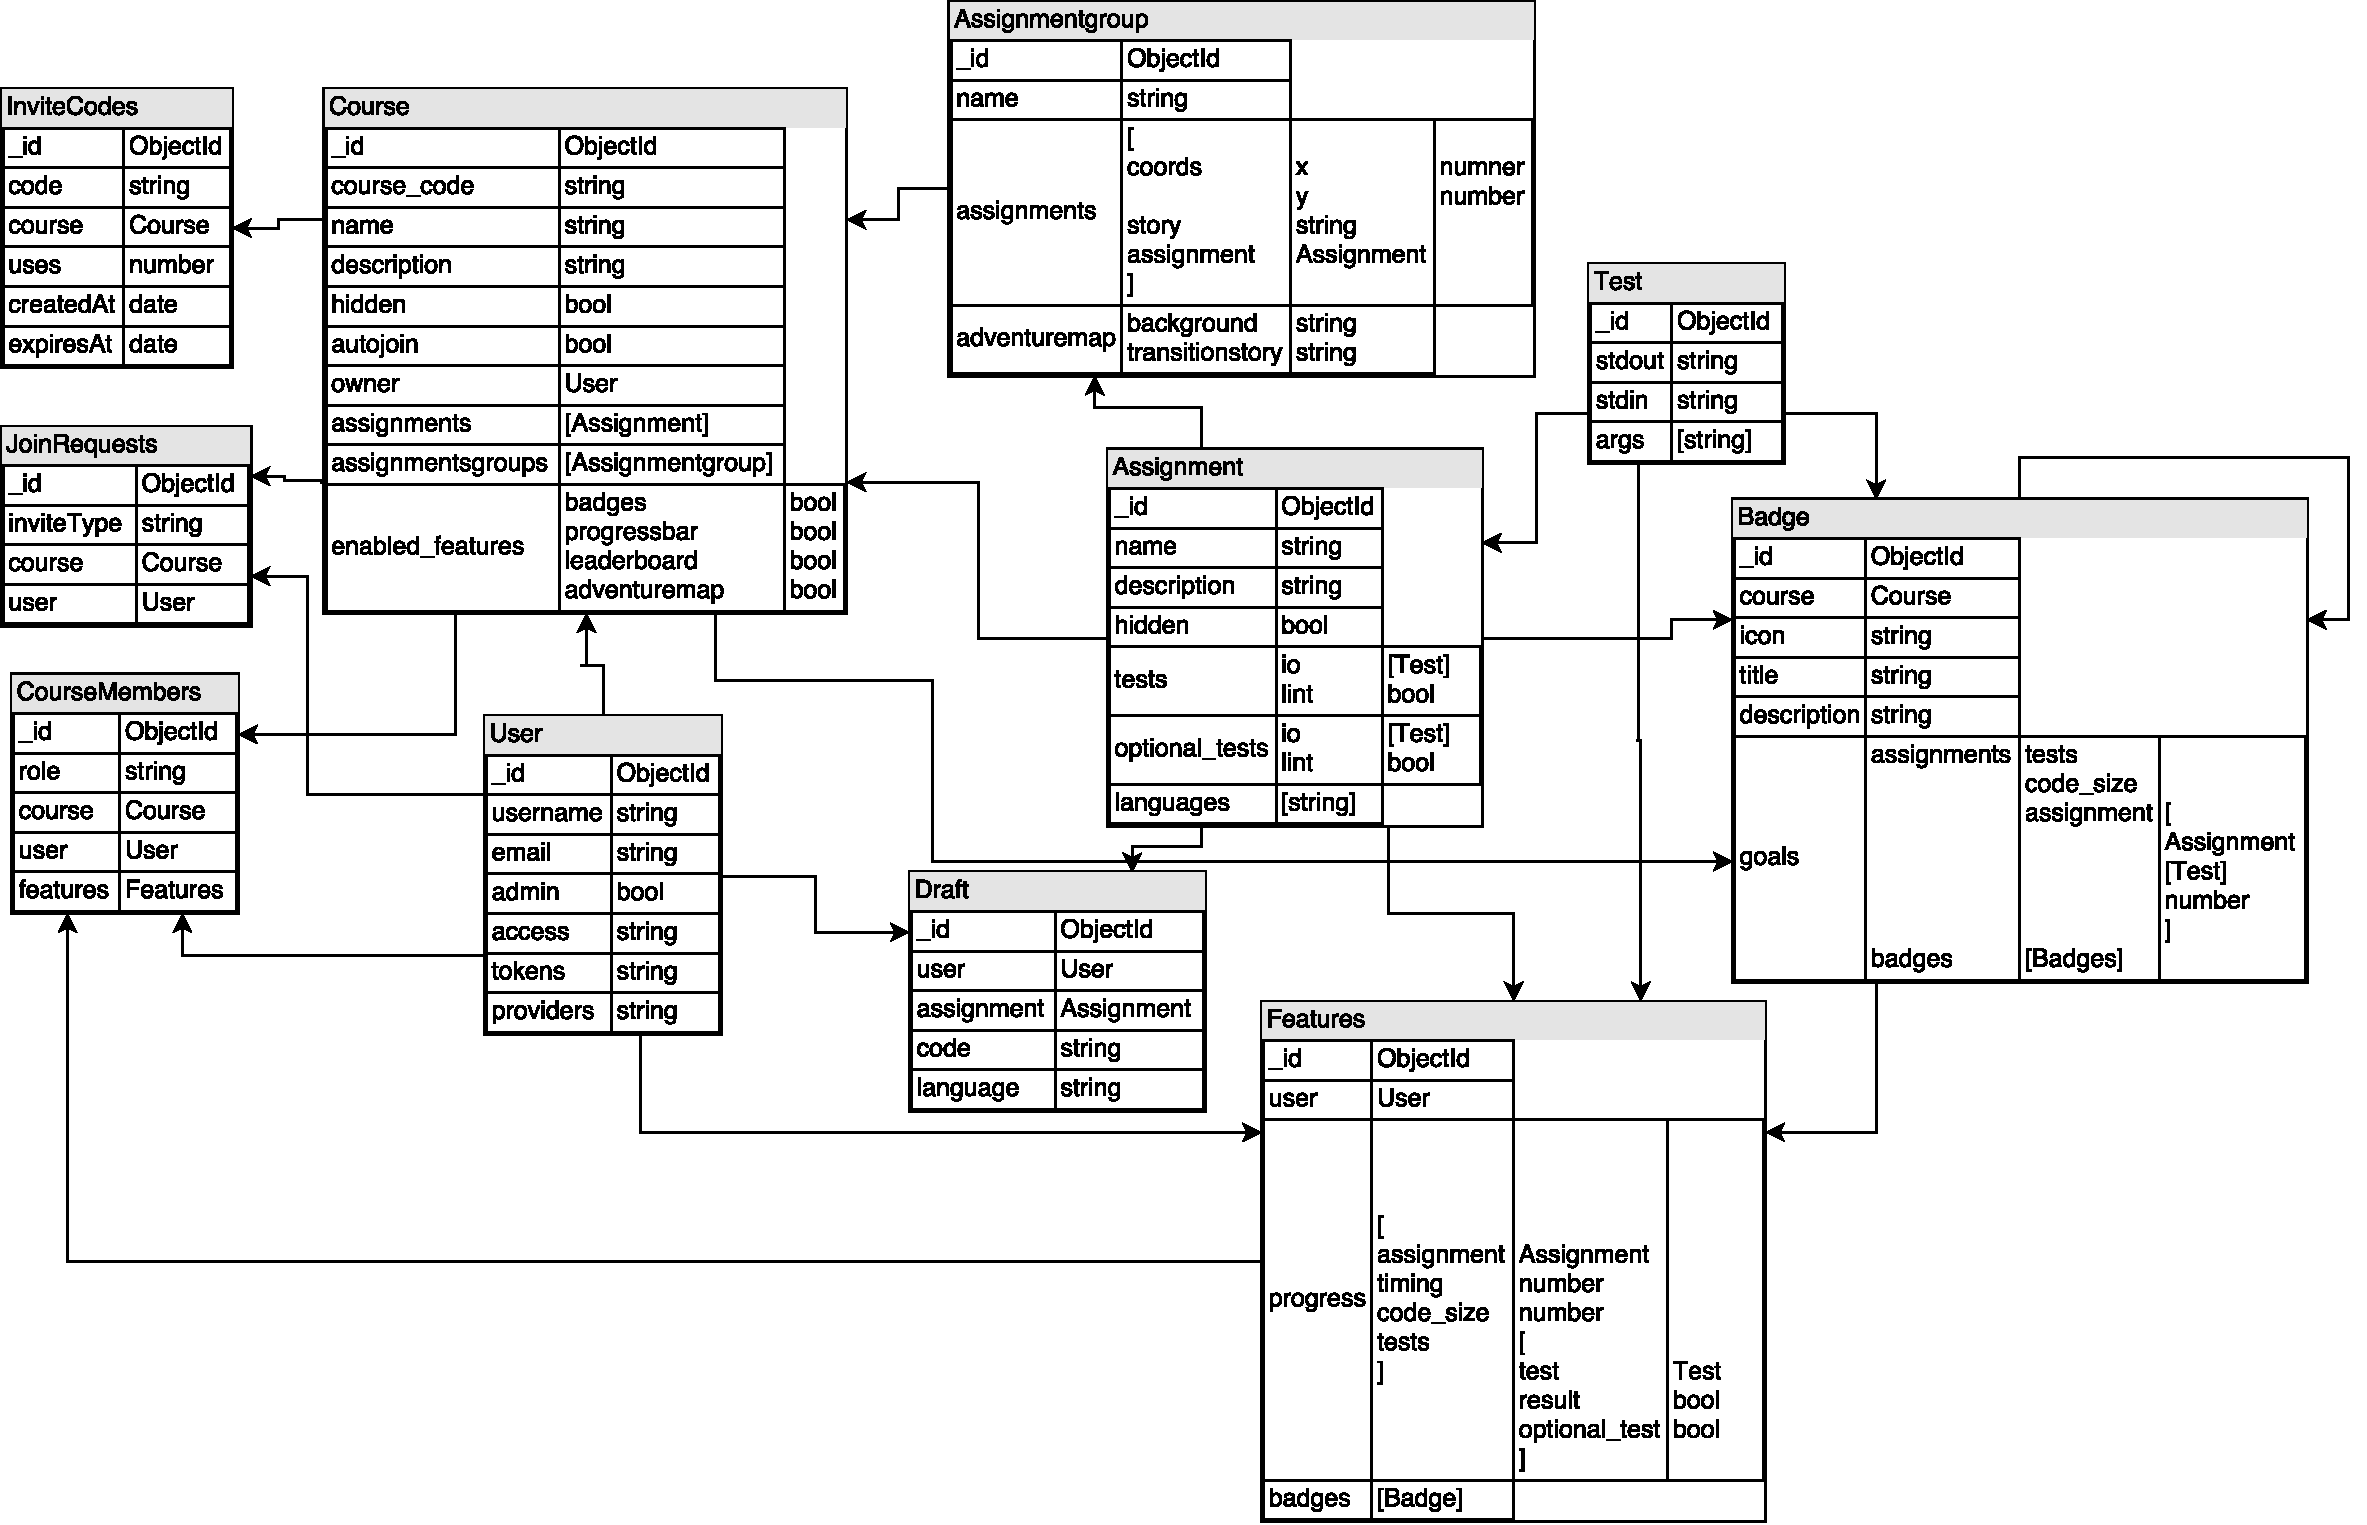
\includegraphics[width=\textwidth]{img/gpp_database-schema.pdf}
    \caption{Overview of the database schema. The arrows point from collections that are referenced to the collections that reference them.}
    \label{fig:schema}
\end{sidewaysfigure}
		
\href{https://www.mongodb.com}{MongoDB} was chosen mainly to complete the MEAN software stack (MongoDB, Express, Angular, \nodejs{}). The majority of the group members working on backend did not have prior experience working with NoSQL databases which presented a good opportunity to learn. MongoDB is a popular choice among NoSQL databases. Mongo uses a JSON-like document structure and JSON is the data format used when different parts of the project services communicate.

\href{http://www.mongoosejs.com}{Mongoose} is a package that extends MongoDB by enforcing a database structure. With Mongoose it's possible to create schemas that describe the format of the data that is to be stored in the database. It was chosen to work with Mongoose because the project members believed it would simplify database interactions, but it also presented a consistency problem to the project. If the Mongoose schemas were updated, there would be a mix of data, some of it stored in the previous format and some in the new. This resulted in a need to either migrate or remove the data in the database after schema updates.

While developing it also proved valuable to have a graphical representation of the data. The data was displayed using \href{https://github.com/mrvautin/adminMongo}{AdminMongo} which also enabled developers to create new entries, edit existing data and delete data. Being able to insert and edit data presented some issues throughout the project since the tool has full freedom when inserting data. No input validation or checks to the current database schemas are made. 

\subsubsection{Schema}
An overview of the database schema can be seen in figure \ref{fig:schema}. There are a number of core collections: \emph{User}, \emph{Course}, \emph{Assignment} and \emph{Test}. These core collections are essential for the base functionality of the platform. The other collections are auxiliary and were added to support additional functionality and features. For example, \emph{Assignmentgroup} makes it possible for teachers to divide course assignments into groups and is used, among other things, to support some gamification elements.

The database design started with the core collections and evolved during development to support new features that were added. Decisions needed to be made quickly to maintain the workflow, which might have resulted in some suboptimal solutions. The resulting schema was very relational, which imposed a problem as MongoDB only supports atomicity on a document level. An example of this is if a document is removed from the database, separate queries need to be made to remove any references held by other documents, which may result in inconsistencies if other queries are made at the same time. The solution to this would be to design a schema with less relations, or to use a relational database.

\subsection{Feature}
As this project focused on adding gamification elements for programming exercises and making programming more fun in general, it was important to include a tool that supports development of future gamification modules. This tool is called \emph{Feature} and is built in such a way that it is possible to easily extend it with more functionality. Feature works by running all of the gamification modules and storing the results of these modules in a Feature collection associated with a student and a course.

Future developers should be able to expand the system with their own gamification elements without having to learn the whole codebase. This flexibility is achieved with a plug-in system that dynamically loads files and runs code on the results from Tester. This was possible by importing all modules inside the features directory. The plug-in modules need to follow a given interface. They have to contain an initiation function and a function that is called once Tester has delivered back results to Backend. 

The initiation function connects to an event listener that triggers once Backend
gets a result back from Tester. When this event is triggered it will call the
function that executes plug-in specific code. It should be noted that if any of the mandatory tests fail then Feature wont run any gamification plug-ins. Once a plug-in is done calculating it can return results that will be sent back to Frontend.

Even if extensibility was of high priority when developing this tool, it was not
possible to fully decouple it from the rest of the codebase. For example, in front of MongoDB, Mongoose is running in order to structure what is stored in the database. This means that if a plug-in needs to store anything in the database, the database schema has to be modified in order to support the desired structure for that plug-in.

Such an example is the gamification element called \emph{Progress}. After
receiving the results from Tester the result is stored in the Feature collection
of that student, resulting in data that describes the progression of that student's advancements throughout the course.

Another example is \emph{Badge}. Each badge contains information that describes the story behind it and also the goals that have to be achieved in order to earn it. This information is defined in a separate model in the database schema. However, in order to be able to track badges that a student of a course has received the Feature model has to be updated as well.

Feature is somewhat decoupled from the rest of the system and therefore one of the easiest parts to understand and extend. To create a new plug-in is very simple, but because most plug-ins need to store something that is associated with a student, the database schema most likely needs to be modified as well.

\subsection{API Protocol}
A decision was made early in the project to adhere to a RESTful API design. Access paths to resources are built from the database schema, see figure~\ref{fig:schema}. For example: in the current database design, each assignment belongs to a course. It is therefore necessary to reference a specific course to access an assignment. Example: \texttt{GET https://.../api/courses/\allowbreak123123123/assignments/456456456/} returns assignment \texttt{456456456} which belongs to course \texttt{123123123}. Each resource name such as \texttt{courses} is in plural. A POST to \texttt{https://.../api/courses} creates a course while a GET request to the same resource returns all courses.

Data can be sent to the backend via both body and URL. Sending data via body is relevant for PUT and POST requests. The information for such requests should be sent as JSON and it should match the format specified in the API documentation. JSON is also the data-type used by the backend to return data, even when the result returned is a status code.

\subsubsection{API Documentation} \label{apidocs}
Documentation for the API can at the time of writing be found at: \\ \texttt{130.240.5.119:18000/docs}. \\
In general it is found where the Backend server is deployed at: \\ \texttt{BACKEND\_IP:PORT/docs}.

% errors
\subsubsection{Error handling}
To enhance a user's experience when working with the API, it was decided that a good way to handle both user errors and server errors should be implemented.

A server error is defined as an unexpected error that could cause the server to crash and therefore become unresponsive. A server error should never prevent the server from continuing serving data from working routes. Therefore every server error is handled and returned to the user as an HTTP error, \texttt{500:\@ Internal server error}. As explained in the logging section~\ref{logging}, a server error is logged to help maintainers localize where things went wrong. This also prevents the server from crashing, but the route which threw the error will still throw the error until it's patched.

A user error is defined as any error caused by a user of the API. Trying to call a non existent route, not including input or including the wrong input are examples of user errors. If such an error is encountered it's important that the user receives feedback on what they are doing wrong. Both a fitting HTTP error code and error message should be returned. If a user has missed one required input field they should be told exactly which field is missing. All user errors are returned with an HTTP error code of 4xx.

Another type of user error occurs when the user makes a valid request which can not be handled because of restrictions implemented in the API. For example, if a user tries to modify data which they don't have access to. These errors are still considered user errors and will follow the error form of such an error.
% extensibility in features/progress/gamification

\subsection{Quality Control}
% jenkins
\subsubsection{Continuous Integration}
As a way to keep the project effective it was determined that it was important to implement continuous integration as a part of the project. This helps to achieve a modern workflow, where changes pushed to the repository are automatically tested and built on a live test server. Using continuous integration was also a good way to separate production and development builds, and a way to ensure that production builds always kept a certain standard and robustness. The solution used was \href{https://jenkins-ci.org/}{Jenkins}, which is well established.

While the idea of how continuous integration was supposed to be used in the project was quite clear, the concept wasn't put to as good use as it could have. In the first half of the project, the builds generated from Jenkins weren't really put to use. This was mainly due to communication errors and the fact that the builds weren't needed as much as expected. For the second part of the project, the builds were used more. The way that the deployment with Jenkins was setup was to build from two branches from Git, one from \texttt{master}, which was supposed to build for production, and another from \texttt{backend}, which was supposed to build for development. The idea was that the development build would always contain the latest changes in \texttt{backend}. As the project reached its deadline it became increasingly important to keep the backend development builds stable because of the fact that the frontend team was depending on the backend development build.

Because of the increasing demands of having stable backend development builds, a new requirement was set up for the continuous integration where a new development build was only built if it passed a set of unit tests.

% different environments
\subsubsection{Different Environments}
Connected to the reasoning of building the backend in different environments/modes, such as production or development, it was important to load different configurations depending on what environment the backend was supposed to run. For example, the production environment should not use the same database as the development environment. Because of this, it was important to be able to run the backend in different modes and dynamically load the correct configurations based on the mode that the backend was running in, hence a system that did this was implemented.

% logging
\subsubsection{Logging} \label{logging}
A large part of the work of development and support teams work is monitoring, debugging and troubleshooting. Because of this it is important to have good logging as a way to make these processes easier, faster and smoother. Having good logging gives a good insight into what the application is doing and how it works. Because of this, it was essential to have proper, useful and extensible logging available in the backend. A custom logging system, named \emph{Logger}, was developed that ran with \href{https://github.com/winstonjs/winston}{Winston} and \href{https://github.com/expressjs/morgan}{Morgan} at its core. Winston is a simple and universal logging library and Morgan is an HTTP request logger middleware. Logger combined Winston and Morgan with the selectiveness of running the backend in different modes/environments. Depending on the mode, Logger had different parts that it logged into log files.

Logger was set up to log all errors, server errors and a general logs in separate log files. When running in development mode it was also important to log to the console, but not otherwise, hence console logging was only enabled when the backend ran in development mode.

Winston and Logger use levels to identify what type of information a log contains. The logging levels in Logger conform closely to the severity ordering specified by RFC6424.
The severity of all levels are numerically ascending from most important to least important.

\begin{enumerate}
  \item Server Error
  \item Error
  \item Warning
  \item Info
  \item Verbose
  \item Debug
  \item Silly
\end{enumerate}

% automated testing
\subsubsection{Automated Testing}
The API is a large part of the backend codebase. Automated tests of the endpoints were developed, mainly to guard against regressions. The tests mostly assert that the server doesn't return an error when given good input. In order to save time in test development, the tests are run in order, where older tests create the resources that are needed for later tests. This is not good practice in automated tests, but it would have been far more costly to make the tests independent of each other by doing setup and teardown for each endpoint test.
